\defChapterTarget[ArchitecturalDesign]{Architectural design}
    \section{\textit{Overview}: High-level components and their interaction}
    The whole software that will become the main core of the SafeStreets
    initiative will be developed as a distributed application, which means that
    the software will be executed (or run) on multiple devices within a network.
    It will have a three-layers logic and be divided as following:
    \begin{itemize}
        \item \textbf{P}: The \textbf{\emph{presentation}} layer will handle all
        \textit{incoming} (\textit{and outcoming}) relations with the customers
        \item \textbf{A}: The \textbf{\emph{application}} layer will work as a
        "man in the middle" between the \textbf{P}resentation layer and the
        \textbf{D}atabase layer and will hold all the needed logic for the
        software to correctly work;
        \item \textbf{D}: The \textbf{\emph{database}} layer will be needed in
        order to store and manage all needed (and requested) information of the
        initiative;
    \end{itemize}
    Each and every one of the layers the architecture will be composed by a
    (group of) machines. By doing this, it is meant to provide, to each layer,
    its own dedicated hardware, for either scalability, failure handling and
    flexibility reasons.\\
    The following image shows the high-level architecture of the system without
    providing any detail of the components which will form the structure of the
    software itself, which will be tackled later in this document.
    \begin{figure}
        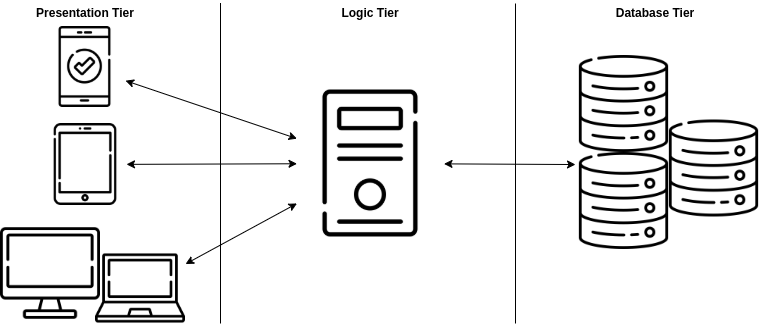
\includegraphics[scale=0.45]{dd/resources/images/HighLevelStructure.png}
        \caption{High-level architecture}        
    \end{figure}

    \section{Component view}
    %inserire immagine component view uml
    \begin{itemize}
        \item \textbf{Router}:it manages messages and function calls coming from
        other subsystems in order to pass the data to the correct element of the
        system. It eventually calls the correspondent method/function on it.
        Furthermore, the router is partitioned according to the type of the
        interacting components because of the different functionalities. 
        \item \textbf{SignUpManager}: this component provides all the procedures
        to allow customers to register to SafeStreets. Obviously, this
        components has also to interact with the DBMS to store the registration
        data and to run a check about the chosen email, password and
        AuthoritiesID or fiscal code.
        \item \textbf{SignInManager}: it contains all the logic devoted to the
        authentication of the customers. It check the authentication parameters
        using the data stored on the DBMS.
        \item \textbf{SignalViolationManager}: it deals with the signalations of
        violations made by the users. This component has to verify that all the
        inserted data are correct and if not has to immediately ask the user to
        provide more information.
        \item \textbf{UnsafeAreasManager}: this component provides all the users
        the possibility to see the unsafe areas. It receives all the information
        from the DBMS.
        \item \textbf{ViolationsListManager}: with this component the user can
        see all the violations he/she has reported. The authority user can see
        all the violations reported in his/her area.
        \item \textbf{ViolationsCheckingManager}: this component provides the authority user 
        \item \textbf{StatisticsManager}: this component provides the authority
        user the possibility to see all the statistic generated crossing the
        data on violations. It receives all the information from the DBMS.
        \item \textbf{CrossDataManager}: it crosses data from SafeStreets
        database and from the municipality database to generate the statistics
        and the unsafe areas.
    \end{itemize}    
    \section{Deployment view}
    The following image is a deployment diagram which represents the
    architecture of the system as distribution(deployment) of software artifacts
    to deployment targets(node). Artifacts represents elements obtained with a
    development process. Nodes can represent either hardware or software environments.
    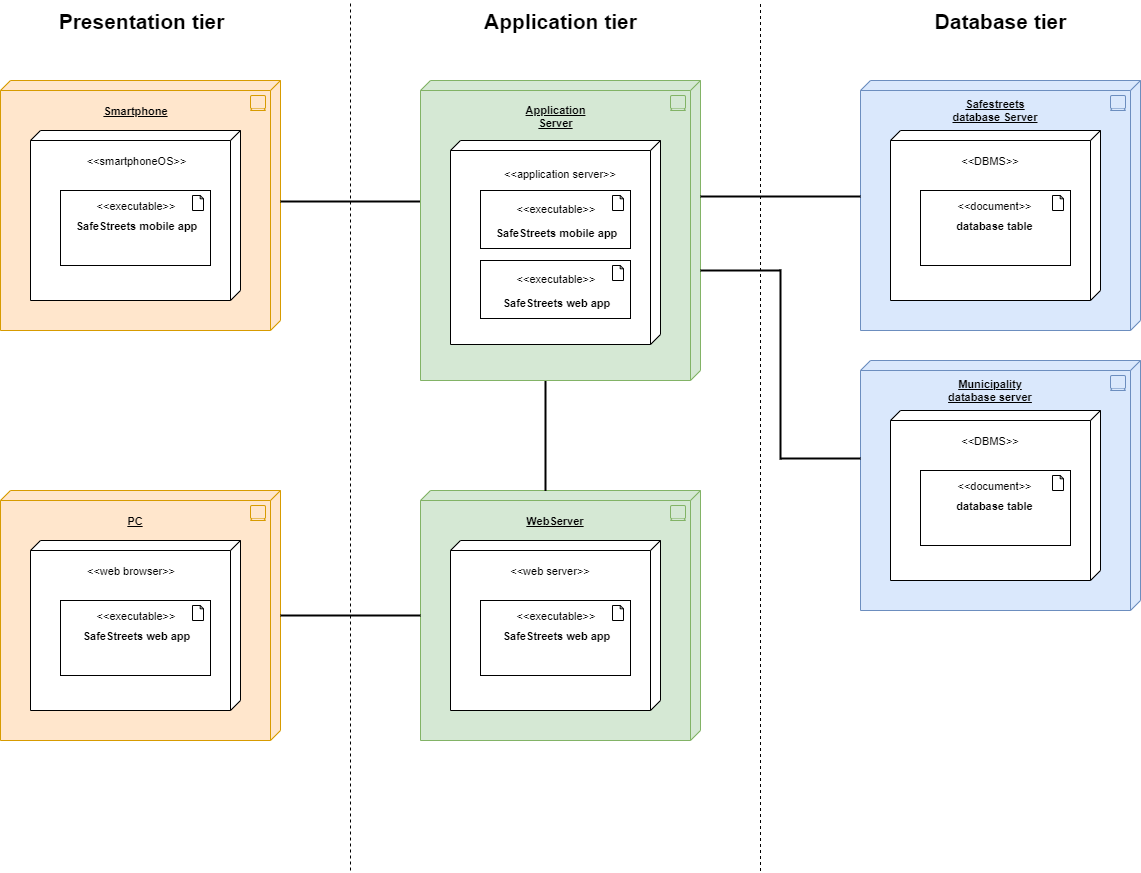
\includegraphics[scale=0.4]{dd/resources/images/Deployment Diagram.png}
    The three tiers contain:
    \begin{itemize}
        \item \textbf{Presentation tier}: in this tier the presentation logic is
        deployed. Users are provided with a mobile application on their mobile
        devices and authority users are provide with both a mobile application
        and a web application accessible from a common browser. The mobile
        application must be developed for most of the devices (both iOS and
        Android version). Both user and authority user ask to communicate to the
        application server in order to retrieve data, signal a violation, check
        violations or unsafe areas.
        \item \textbf{Application tier}: in this thier the application logic is
        deployed. The application server allows the mobile application and the
        web application to access data stored into the SafeStreets database. The
        application server also implements the business logic and handles the
        requests. The mobile application directly addresses the application
        server. The web server allow authority users to use SafeStreets
        services. If it can't provide some information it forwards the requests
        to the application server.
        \item \textbf{Database tier}: in this tier data access must be deployed.
        The application has to handle data both on SafeStreets database and on
        the municipality database for cross references.
    \end{itemize}    
    \section{Run-time view}
        \subsection{Synchronization}
        \subsection{Request data regarding a group of people}
        \subsection{Request data regarding a particular user by providing his/her UUID}
    \section{Component interface}
    \section{Selected architectural styles and patterns}    
        \subsection{Design Patterns}
            \subsubsection*{Model View Controller (MVC)}
    \section{Other design decisions}